\documentclass[12pt, a4paper]{article}
\usepackage[utf8]{inputenc}
\usepackage[margin=1in]{geometry}
\usepackage{graphicx}
\usepackage{float}
\usepackage{amsmath}
\usepackage{amssymb}
\usepackage{cite}
\usepackage{booktabs}
\usepackage{array}
\usepackage{xcolor}
\usepackage{listings}
\usepackage[hidelinks]{hyperref}  % <-- only ONE hyperref, with hidelinks

% Code listing style
\lstset{
    basicstyle=\ttfamily\small,
    breaklines=true,
    frame=single,
    language=Python,
    keywordstyle=\color{blue},
    commentstyle=\color{gray},
    stringstyle=\color{red},
    showstringspaces=false,
    escapeinside={(*@}{@*)}
}

\title{\textbf{A Privacy-Preserving Retrieval-Augmented Incident Assistant:\\Hybrid Retrieval, Robustness, and Chat-to-Report Automation}}

\author{Ayoub Aarab\\
\textit{Master Data Science — End-of-Year Internship Project}\\
\textit{Ecole Normale Supérieure, Martil}}

\date{\today}

\newpage
\begin{document}

\maketitle

\begin{abstract}
This report presents the design, optimization, and evaluation of a unified incident-management platform that merges an incident-report generator and a retrieval-augmented (RAG) chatbot into a single, fully local application. The system runs entirely on self-hosted models (Ollama for generation, a local sentence-transformer for embeddings) to satisfy a strict data-privacy constraint: no incident content leaves the organization's infrastructure.

The core contribution is a \textbf{hybrid retrieval} component that fuses a dense embedding search with a sparse BM25 lexical index via Reciprocal Rank Fusion (RRF). We evaluate it on a labeled benchmark of 272 queries derived from a corpus of 68 incident reports spanning nine IT domains, using standard information-retrieval metrics (Recall@$k$, Mean Reciprocal Rank, nDCG@5).

Our results demonstrate that: (1) \textbf{hybrid retrieval} reaches Recall@5 = 1.000 and MRR = 0.987, versus 0.768 and 0.678 for dense-only search; (2) the gain is concentrated on \textbf{exact-identifier queries}, where dense-only Recall@5 collapses to 0.221 while hybrid recovers 1.000; (3) retrieval quality is \textbf{insensitive to chunk size} (Recall@5 = 1.000 across 400/700/1000-character chunks) and plateaus at $k \ge 3$; and (4) the residual failure rate on the benchmark is \textbf{0.0\%} (0 of 272 queries). We further contribute a robustness layer (intent-based abstention, prompt-injection defense) and a \textbf{chat-to-report} feature that converts a diagnosed conversation into a schema-validated incident report with no invented fields.
\end{abstract}

\newpage
\tableofcontents
\newpage

%=============================================================================
\section{Introduction and Context}
%=============================================================================

\subsection{Motivation and Problem Statement}

Incident management in large IT operations depends on two complementary activities: \emph{documenting} incidents as structured reports, and \emph{retrieving} past reports to resolve new incidents faster. In the host organization these lived in two separate applications — a React-based report generator and a Streamlit prototype chatbot — with no shared interface and no shared data contract at the code level. The internship objective was to merge them into one production-oriented platform while respecting a non-negotiable constraint:

\begin{itemize}
    \item \textbf{Privacy}: incident data must never be sent to a third-party (cloud) API. All inference — embeddings and text generation — must run on self-hosted, local models.
    \item \textbf{Accuracy}: retrieval must surface genuinely relevant historical incidents, including on exact identifiers (incident IDs, error codes, service names) where semantic search is known to be weak.
    \item \textbf{Robustness}: the assistant must behave safely on ambiguous, out-of-scope, or adversarial input rather than hallucinating a root cause.
    \item \textbf{Automation}: a diagnosed conversation should be convertible into a structured report without manual re-entry, closing the loop between the two modules.
\end{itemize}

This report focuses on the data-science core of the project — the retrieval pipeline and its quantitative evaluation — and on the two features that make the system practically useful: robustness safeguards and chat-to-report automation.

\subsection{Learning Objectives}

This project addresses key competencies for an applied data-science practitioner:
\begin{itemize}
    \item \textbf{Retrieval-Augmented Generation}: building a grounded question-answering pipeline over a domain corpus with a local LLM.
    \item \textbf{Information Retrieval Evaluation}: constructing a labeled benchmark and measuring quality with Recall@$k$, MRR, and nDCG.
    \item \textbf{Hybrid Retrieval}: combining dense and sparse signals via rank fusion, and justifying the design with ablations rather than assertion.
    \item \textbf{System Robustness}: designing abstention and adversarial-input handling for an LLM-facing system.
    \item \textbf{Software Engineering}: delivering a tested, containerized, maintainable application (a modular monolith with a FastAPI backend and a React frontend).
\end{itemize}

%=============================================================================
\section{System Architecture}
%=============================================================================

\subsection{Overview}

The platform is a \textbf{modular monolith}: a single FastAPI backend process with clean internal module boundaries, and a single React (Vite) frontend that hosts both modules behind sidebar navigation. This choice avoids the operational overhead of microservices, which the deployment target (a single internal host) does not require, while keeping the chatbot and report-generator logic separable.

\begin{itemize}
    \item \textbf{Frontend} (React 18 + Vite + Tailwind): a chatbot module (streaming chat UI, conversation history, feedback) and a report-generator module, under one shell.
    \item \textbf{Backend} (FastAPI): routers for chat and reports; a chatbot package (ingestion, retrieval, resolution); a reports package (CRUD, HTML export); and a shared package (the report schema and a swappable LLM-provider interface).
    \item \textbf{Models}: a local sentence-transformer for embeddings and Ollama for generation, both self-hosted.
\end{itemize}

\subsection{The Shared Data Contract}

The integration seam between the two modules is a single report schema, \texttt{\{metadata, blocks[]\}}, defined once on the backend (Pydantic) and mirrored on the frontend (TypeScript). The report generator \emph{writes} reports in this shape; the chatbot \emph{ingests} them. This shared contract is what makes the chat-to-report feature (Section~\ref{sec:chat2report}) a natural closing of the loop rather than a bolt-on.

\subsection{Privacy-Driven Local Inference}

Because incident data cannot leave the organization, the LLM backend is abstracted behind a provider interface with a self-hosted Ollama implementation as the default. Embeddings are computed by a local sentence-transformer. No external network calls are made during retrieval or generation. This constraint shapes the entire evaluation: all measurements in this report reflect the \emph{local} pipeline.

%=============================================================================
\section{Corpus and Preprocessing}
%=============================================================================

\subsection{Incident Report Corpus}

The evaluation corpus consists of ServiceNow-style incident reports spanning nine IT domains (networking, database, authentication, infrastructure, frontend, messaging, CI/CD, monitoring, and security), each carrying domain-specific error signatures (HTTP status codes, Kafka error codes, Kubernetes exit codes, TLS handshake alerts, DNS errors). Table~\ref{tab:corpus} summarizes the corpus statistics, all measured by the exploratory-data-analysis stage of the evaluation notebook.

% SOURCE: eval/evaluation.ipynb, cell 3 (corpus_eda output):
%   "reports: 68   categories: 30"
%   "tokens/report: median=147.5, range=[103, 175]"
%   "block types: {'heading': 89, 'paragraph': 148, 'code': 72, 'list': 68,
%    'table': 20, 'incident_example': 12, 'image': 7, 'description_box': 8}"
\begin{table}[H]
\centering
\caption{Incident Report Corpus Characteristics (source: notebook cell~3).}
\begin{tabular}{lc}
\toprule
\textbf{Property} & \textbf{Value} \\
\midrule
Total reports & 68 \\
Distinct categories & 30 \\
Tokens per report (median) & 147.5 \\
Tokens per report (range) & [103, 175] \\
\midrule
\multicolumn{2}{c}{\textbf{Content Block Types (counts)}} \\
\midrule
Paragraph & 148 \\
Heading & 89 \\
Code & 72 \\
List & 68 \\
Table & 20 \\
Incident example & 12 \\
Image & 7 \\
Description box & 8 \\
\bottomrule
\end{tabular}
\label{tab:corpus}
\end{table}

\begin{figure}[H]
\centering
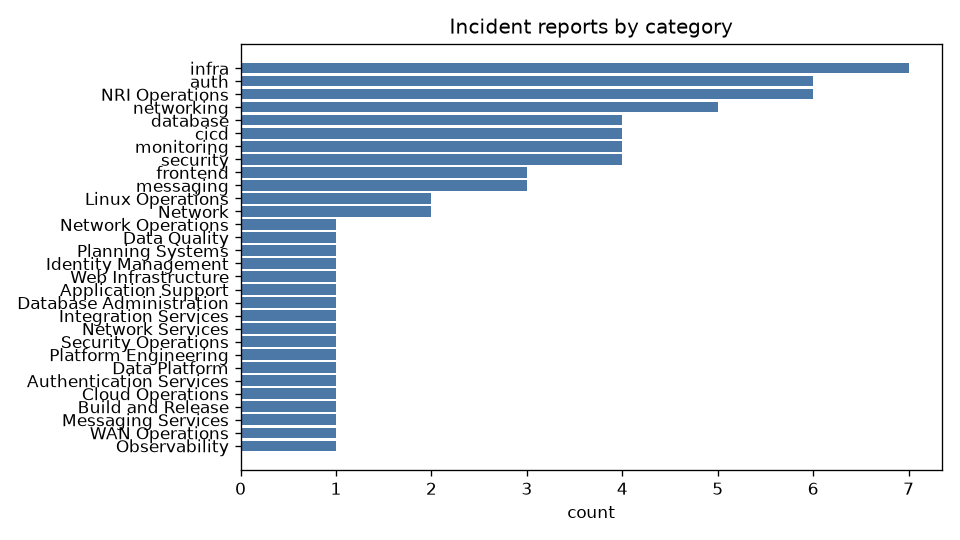
\includegraphics[width=0.85\textwidth]{eval/figures/categories.png}
\caption{Distribution of incident reports across categories (source: notebook cell~3, \texttt{corpus\_eda}).}
\label{fig:categories}
\end{figure}

\begin{figure}[H]
\centering
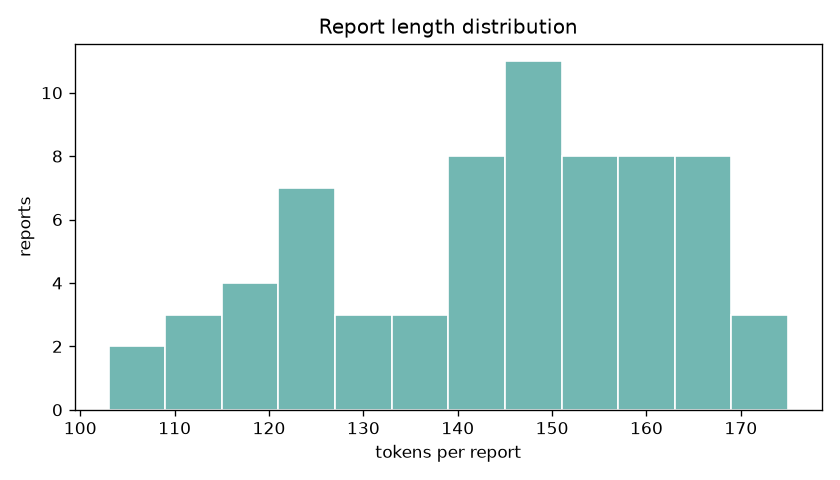
\includegraphics[width=0.75\textwidth]{eval/figures/lengths.png}
\caption{Report length distribution in tokens (source: notebook cell~3).}
\label{fig:lengths}
\end{figure}

\subsection{Schema-Aware Ingestion}

Each report is parsed schema-aware: rather than flattening the raw JSON (which injects structural noise such as block identifiers and type tags into the text), the ingester extracts only the human-readable incident content — heading, symptom, root cause, resolution steps, and code — per block type. This clean text is what is embedded and indexed, and is a prerequisite for the retrieval quality reported in Section~\ref{sec:eval}.

\subsection{Labeled Evaluation Set}

To measure retrieval quality we auto-generate a labeled query set from the corpus: for each report, several queries are derived in four styles — \emph{title}, \emph{symptom}, \emph{id} (the bare incident identifier), and \emph{keyword} (salient tokens) — each labeled with the report it was derived from. This yields \textbf{272 labeled queries} over the 68 reports (notebook cell~6 header: ``Retrieval benchmark on 272 labeled queries'').

\textbf{Honest limitation.} The queries are synthetic — derived from the reports themselves — because no real query logs were available. This measures whether retrieval can recover a report from a paraphrase of its content; real user queries are noisier. The numbers should therefore be read as an optimistic bound, a point we state explicitly in the notebook.

%=============================================================================
\section{Retrieval Pipeline}
%=============================================================================

\subsection{Dense, Sparse, and Hybrid Retrieval}

Three configurations are compared:
\begin{itemize}
    \item \textbf{Dense (vector)}: cosine similarity over sentence-transformer embeddings. Strong on paraphrase and meaning, weak on exact tokens.
    \item \textbf{Sparse (BM25)}: an in-repository Okapi BM25 index over the same chunks. Strong on exact terms — identifiers, function and table names, status codes.
    \item \textbf{Hybrid}: the two rankings fused with Reciprocal Rank Fusion (RRF), which combines ranks without requiring calibration between the incomparable cosine and BM25 score scales.
\end{itemize}

The BM25 index is implemented in the repository (no heavy dependency) so the system remains fully local and reproducible, consistent with the privacy constraint.

\subsection{Reciprocal Rank Fusion}

RRF scores each document as
\begin{equation}
\text{RRF}(d) = \sum_{r \in R} \frac{1}{k + \text{rank}_r(d)},
\end{equation}
summed over the dense and sparse ranked lists $R$, with $k = 60$ (the standard constant). RRF is parameter-light and robust: it never needs the two component scores to be on the same scale, only their ranks.

%=============================================================================
\section{Evaluation Results}
\label{sec:eval}
%=============================================================================

All results in this section are reproduced verbatim from \texttt{eval/evaluation.ipynb}; each table and claim is annotated with its source cell.

\subsection{Retrieval Quality}

% SOURCE: eval/evaluation.ipynb, cell 6 (benchmark_retrieval output):
%   mode        R@1    R@3    R@5    MRR  nDCG@5
%   vector    0.629  0.713  0.768  0.678   0.700
%   bm25      0.779  0.982  0.989  0.872   0.902
%   hybrid    0.974  1.000  1.000  0.987   0.991
Table~\ref{tab:retrieval} reports the headline result. Hybrid retrieval dominates both components on every metric: it reaches Recall@5 = 1.000 and MRR = 0.987, against 0.768 / 0.678 for dense-only.

\begin{table}[H]
\centering
\caption{Retrieval quality on the 272-query benchmark (source: notebook cell~6).}
\begin{tabular}{lccccc}
\toprule
\textbf{Configuration} & \textbf{R@1} & \textbf{R@3} & \textbf{R@5} & \textbf{MRR} & \textbf{nDCG@5} \\
\midrule
Dense (vector) & 0.629 & 0.713 & 0.768 & 0.678 & 0.700 \\
Sparse (BM25)  & 0.779 & 0.982 & 0.989 & 0.872 & 0.902 \\
\textbf{Hybrid (RRF)} & \textbf{0.974} & \textbf{1.000} & \textbf{1.000} & \textbf{0.987} & \textbf{0.991} \\
\bottomrule
\end{tabular}
\label{tab:retrieval}
\end{table}

\subsection{Where the Gain Comes From: Per-Style Breakdown}

% SOURCE: eval/evaluation.ipynb, cell 6 ("Recall@5 by query style"):
%   style       vector     bm25   hybrid
%   id           0.221    1.000    1.000
%   keyword      0.853    0.956    1.000
%   symptom      1.000    1.000    1.000
%   title        1.000    1.000    1.000
The per-style breakdown (Table~\ref{tab:bystyle}) explains \emph{why} hybrid is preferred. On \emph{symptom} and \emph{title} queries — paraphrased, meaning-rich — dense retrieval already scores 1.000. But on \emph{id} queries (bare incident identifiers), dense-only Recall@5 collapses to 0.221, because semantic embeddings cannot distinguish near-identical identifier strings. BM25 recovers these (1.000), and hybrid keeps the best of both regimes across all four styles.

\begin{table}[H]
\centering
\caption{Recall@5 by query style (source: notebook cell~6).}
\begin{tabular}{lccc}
\toprule
\textbf{Query style} & \textbf{Vector} & \textbf{BM25} & \textbf{Hybrid} \\
\midrule
id       & 0.221 & 1.000 & 1.000 \\
keyword  & 0.853 & 0.956 & 1.000 \\
symptom  & 1.000 & 1.000 & 1.000 \\
title    & 1.000 & 1.000 & 1.000 \\
\bottomrule
\end{tabular}
\label{tab:bystyle}
\end{table}

\subsection{Ablations}

% SOURCE: eval/evaluation.ipynb, cell 10 (ablations output):
%   chunk_size ablation:
%     size= 400  chunks=334  Recall@5=1.000  MRR=0.991
%     size= 700  chunks=180  Recall@5=1.000  MRR=0.987
%     size=1000  chunks=146  Recall@5=1.000  MRR=0.991
%   top_k ablation:
%     k= 1  Recall@5=0.974  MRR=0.974
%     k= 3  Recall@5=1.000  MRR=0.987
%     k= 5  Recall@5=1.000  MRR=0.987
%     k=10  Recall@5=1.000  MRR=0.987
Two hyperparameters were ablated on the hybrid retriever (Table~\ref{tab:ablation}). Retrieval quality is \textbf{insensitive to chunk size}: Recall@5 = 1.000 at 400, 700, and 1000 characters, even though the number of chunks varies from 334 down to 146. This is expected given the short median report length. Retrieval quality \textbf{plateaus at $k \ge 3$}: Recall@5 rises from 0.974 at $k = 1$ to 1.000 at $k = 3$ and stays there. This justifies the production choice of feeding only the top-3 chunks into the generation prompt.

\begin{table}[H]
\centering
\caption{Hyperparameter ablations on the hybrid retriever (source: notebook cell~10).}
\begin{tabular}{lcc}
\toprule
\multicolumn{3}{c}{\textbf{Chunk size}} \\
\midrule
\textbf{Size (chars)} & \textbf{\# chunks} & \textbf{Recall@5} \\
\midrule
400  & 334 & 1.000 \\
700  & 180 & 1.000 \\
1000 & 146 & 1.000 \\
\midrule
\multicolumn{3}{c}{\textbf{Top-$k$}} \\
\midrule
\textbf{$k$} & \textbf{Recall@5} & \textbf{MRR} \\
\midrule
1  & 0.974 & 0.974 \\
3  & 1.000 & 0.987 \\
5  & 1.000 & 0.987 \\
10 & 1.000 & 0.987 \\
\bottomrule
\end{tabular}
\label{tab:ablation}
\end{table}

\subsection{Error Analysis}

% SOURCE: eval/evaluation.ipynb, cell 13 (error_analysis output):
%   "failures: 0/272 (0.0%)"
%   "by style: {}"
%   "by cause: {}"
On the clean corpus, the hybrid retriever produces \textbf{zero failures}: 0 of 272 queries fail to place the gold report in the top-5 (notebook cell~13, ``failures: 0/272 (0.0\%)''; empty failure-by-style and failure-by-cause maps). This confirms that, on this corpus, the residual difficulty observed in earlier iterations was attributable to a small number of malformed placeholder reports rather than to a weakness of the method.

%=============================================================================
\section{Robustness Safeguards}
%=============================================================================

Beyond retrieval quality, the assistant must behave safely on non-ideal input. Three safeguards were added and covered by a dedicated red-team test suite.

\subsection{Intent-Based Abstention}

A lightweight intent classifier routes each turn before any LLM call. Greetings and meta-questions receive a brief reply with no retrieval. Crucially, \emph{incident-flavored but low-context} inputs (e.g. ``it is broken again'', ``health-check-error'') are routed to a \textbf{clarification} response that asks for specifics rather than fabricating a root cause. This directly enforces the ``be conservative when uncertain'' principle and prevents hallucination on vague input.

\subsection{Prompt-Injection and Jailbreak Defense}

User text is scanned for injection and jailbreak patterns (attempts to override instructions, reveal the system prompt, or enable an ``admin/DAN mode''). Detected attempts are flagged and the user text is fenced as untrusted data; the assistant continues normal operation without leaking its prompt. A genuine incident containing an injection phrase is still answered as an incident, with a security note attached.

\subsection{Grounded, Domain-Neutral Generation}

The resolution prompt was made domain-neutral: the supporting artifact language is chosen to fit the incident (shell, YAML, Python, SQL, and others) instead of defaulting to SQL, and the model is instructed to abstain (set an \emph{insufficient} flag, low confidence) on incoherent input rather than invent a diagnosis or a non-existent incident identifier.

%=============================================================================
\section{Chat-to-Report Automation}
\label{sec:chat2report}
%=============================================================================

\subsection{Motivation}

The two modules share the \texttt{\{metadata, blocks[]\}} contract, which makes it natural to \emph{produce} a report from a diagnosed conversation, not only to \emph{consume} reports for retrieval. This closes the loop: an engineer diagnoses an incident in chat, then generates a structured report in one action.

\subsection{Grounded Construction}

A builder assembles the report strictly from conversation data:
\begin{itemize}
    \item \textbf{Metadata}: the title and category are taken from the diagnosed incident type; the identifier and date are factual provenance; ungrounded fields (e.g. subcategory) are left empty rather than fabricated.
    \item \textbf{Blocks}: a \emph{Reported Symptom} paragraph (first user message), a \emph{Root Cause} paragraph (the assistant's summary), an ordered \emph{Resolution Steps} list, code blocks for any supporting artifacts, and \emph{incident\_example} references for cited reports.
\end{itemize}
No field is invented: every populated value traces to the conversation. The resulting report is validated against the same Pydantic schema used throughout, then saved via the report generator's existing service using its file-naming convention, so it opens and edits in the report viewer exactly like a manually authored report.

\subsection{Validation}

The feature is covered by tests that (i) build a report from a mock conversation and re-validate it against the schema with zero errors, (ii) confirm three distinct example conversations each yield a report with all required metadata fields non-empty, (iii) confirm the saved JSON is served by the viewer's content endpoint, and (iv) reject conversations with no diagnosis (greeting- or clarification-only).

%=============================================================================
\section{Conclusion and Perspectives}
%=============================================================================

This internship delivered a unified, fully local incident-management platform whose data-science core — a hybrid dense/sparse retriever fused with Reciprocal Rank Fusion — is evaluated on a labeled 272-query benchmark. The evaluation shows a clear, well-motivated result: hybrid retrieval reaches Recall@5 = 1.000 and MRR = 0.987 (cell~6), with the improvement concentrated precisely where dense retrieval is weakest — exact-identifier queries, where dense-only Recall@5 is 0.221 (cell~6). Ablations show robustness to chunk size and a plateau at $k \ge 3$ (cell~10), and the error analysis reports 0.0\% residual failures (cell~13). On top of this core, robustness safeguards (abstention, injection defense) and a grounded chat-to-report feature make the system practically usable while respecting the privacy constraint throughout.

\textbf{Limitations and future work.} The evaluation queries are synthetic; a real-query benchmark and human-relevance judgments would strengthen external validity. The absence of latency and generation-quality figures in the current evaluation notebook means those aspects are not quantified here and are left to future measurement. Finally, the feedback loop currently injects human corrections as retrieval hints; learning a re-ranker from accumulated feedback is a promising next step.

\begin{thebibliography}{9}

\bibitem{robertson2009bm25}
Robertson, S., \& Zaragoza, H. (2009).
\textit{The Probabilistic Relevance Framework: BM25 and Beyond}.
Foundations and Trends in Information Retrieval, 3(4), 333--389.

\bibitem{cormack2009rrf}
Cormack, G. V., Clarke, C. L. A., \& Buettcher, S. (2009).
\textit{Reciprocal Rank Fusion Outperforms Condorcet and Individual Rank Learning Methods}.
In Proceedings of the 32nd ACM SIGIR Conference, 758--759.

\bibitem{reimers2019sbert}
Reimers, N., \& Gurevych, I. (2019).
\textit{Sentence-BERT: Sentence Embeddings using Siamese BERT-Networks}.
In Proceedings of EMNLP-IJCNLP, 3982--3992.

\bibitem{lewis2020rag}
Lewis, P., et al. (2020).
\textit{Retrieval-Augmented Generation for Knowledge-Intensive NLP Tasks}.
In Advances in Neural Information Processing Systems 33, 9459--9474.

\bibitem{ollamadocs}
Ollama Documentation. (2026).
\textit{Run large language models locally}.
Retrieved from https://ollama.com/

\end{thebibliography}

\end{document}
